%%%%%%%%%%%%%%%%%%%%%%%%%%%%%%%%%%%%%%%%%%%%%%%%%%%%%%%%%%%%%%%%%%%%%%%
%%%%  Load the document class and packages                         %%%%
%%%%%%%%%%%%%%%%%%%%%%%%%%%%%%%%%%%%%%%%%%%%%%%%%%%%%%%%%%%%%%%%%%%%%%%
\documentclass[a4paper]{report}
\usepackage{epsfig}            % to insert PostScript figures
\graphicspath{ 
  {figures/} 
}

%Change figure names
\renewcommand{\figurename}{Fig}

\usepackage[bf,footnotesize]{caption} % make captions small and label bold


\addtocounter{chapter}{1} %Because starting at zero is silly
\makeatletter
\renewcommand{\thesection}{\@arabic\c@section}
\renewcommand{\thefigure}{\@arabic\c@figure}
\makeatother

\usepackage[a4paper,margin=2.7cm,tmargin=2.5cm,bmargin=2.5cm]{geometry} 
\usepackage{textcomp}          % To make nice degree symbols and others\usepackage[bf,footnotesize]{caption} % make captions small and label bold
\usepackage{wrapfig}
%to produce the clickable references along the left in Acroread. This
%package must be included last. 
\usepackage[ps2pdf,bookmarks=TRUE]{hyperref} 



%%%%%%%%%%%%%%%%%%%%%%%%%%%%%%%%%%%%%%%%%%%%%%%%%%%%%%%%%%%%%%%%%%%%%%%
%%%%  Hypertext references for Acrobat                             %%%%
%%%%%%%%%%%%%%%%%%%%%%%%%%%%%%%%%%%%%%%%%%%%%%%%%%%%%%%%%%%%%%%%%%%%%%%
\hypersetup{
pdfauthor = {TENSS},
pdftitle = {Optics Exercises},
pdfkeywords = {optics, lenses, refraction, reflection, dispersion,
  telescope, microscope},
pdfcreator = {LaTeX with hyperref},
pdfproducer = {dvips + ps2pdf}
           }


\begin{document}




%set the number of sectioning levels 
\setcounter{secnumdepth}{2}

\begin{center}
\textbf{\Large{Optics Bench Exercises}}
\end{center}

\section{Introduction}
These exercises are designed to teach the basic principles of optics and image formation.
The exercises are aimed at microscope users who want to learn more about their equipment
\footnote{This document was originally written by Francesca Anselmi for a CSHL graduate course.
It was then modified for use at TENSS (www.tenss.ro) by Priyanka Gupta and Adriana Dabacan. 
The present version was created in 2016 by Rob Campbell for an imaging course at the Biozentrum, Basel.}.
The goal of the exercises is to nurture an understanding of image formation, conjugate planes, and how multiple lenses interact in simple optical set ups. 
This hand-out is not standalone and is intended to be delivered alongside a suitable lecture on the topic.
Exercises work best with no more than three people per group.
It is helpful to have the free \textbf{ray optics simulator} from the Google Play store running on a computer when going through the exercises. 

\section{Parts list}
It is possible to carry out the practicals with a variety of different lenses and equipment. 
The assumed parts list is described here, but the same exercises can be carried out with similar parts. 
All parts are purchased from ThorLabs.
Imperial part numbers are listed but metric parts are also available. 
Each set up comprises the following components:


\subsubsection{General optomechanics}
\begin{itemize}
\setlength\itemsep{0.15em}
\item One \textbf{XT66DP-1000} optical rail and ten \textbf{XT66C4} clamping platforms
\item Lens holders: four \textbf{LMR2}, three \textbf{CP02}
\item Two packs of post holders \textbf{PH50-P5}.
\item Post packs (one of each): \textbf{TR30/P5}, \textbf{TR40/P5}, \textbf{TR50/P5}.
\item Screen or filter holder: \textbf{DH1}
\item Translatable slide holder \textbf{XYFM1} (optional)
\item Linear translation stage for focusing: \textbf{SM1Z} (optional)
\item \textbf{RA180} and \textbf{RA90} post clamps.
\end{itemize}


\subsubsection{Optics}
\begin{itemize}
\setlength\itemsep{0.15em}
\item LED Collector lens: 1'', $f=25 mm$ \textbf{LB1761} or $f=30~mm$ \textbf{LA1805}
\item Field Lens/Condenser Lens: 2'', $f=60 mm$ \textbf{LA1401} (two)
\item $f=100~mm$ \textbf{LA1050}, $f=300 mm$ \textbf{LA1256}, $f=200 mm$ \textbf{LA1979}
\item $f=300~mm$ achromatic doublet (\textbf{AC508-300-A}). Optional.
\item $f=-50 mm$ \textbf{LC1715}
\item Olympus 4X objective (\textbf{WD RMS4X}) and RMS to SM1 coupler (\textbf{SM1A3}).
\end{itemize}

\subsubsection{Misc}
\begin{itemize}
\setlength\itemsep{0.15em}
\item Two post mounted iris diaphragms (\textbf{ID25}). 
\item Epoxy-Encased LEDs, 525 nm, 7 mW (\textbf{LED528EHP}).
You will need to chop off the rounded end of the LED, so it doesn't act like a lens.  
A razor blade and very fine polishing paper work for this. Alternatively, find bright non-domed (flat) LEDs.
\item LED mount \textbf{S1LEDM}
\item A 1'' SM1 tube (\textbf{SM1L10}) to make it easier to place the 25 mm lens near the LED.
\item A power source for the LED. e.g. a 5V source and $200\Omega$ resistor. 
\item A laser pointer that fits into an RA90 post clamp. 
\item Coverslips and a marker pen.
\item Slides to image. Golgi stained brain slices work well. 
Failing that, you could by a `toy' slide kit like that supplied by Celestron. 
Electron microscopy grids of known pitch might be useful but aren't explicitly used in these exercises.
\item A tape measure and ruler. 
\end{itemize}

\subsubsection{Tools}
\begin{itemize}
\setlength\itemsep{0.15em}
\item Lens wrenches for SM1 and SM2: \textbf{SPW606} and \textbf{SPW604}
\item Hex keys such as \textbf{CCHK} or \textbf{TC2} (\textbf{TC3} for metric). 
\end{itemize}

\subsubsection{In addition}
In addition to the above, you will need the following items that can be shared across multiple set ups.
\begin{itemize}
\setlength\itemsep{0.15em}
\item Cap screw kit \textbf{HW-KIT2}
\end{itemize}


\clearpage

\section{Image Formation}
An image is formed when all light rays leaving one point (or region) of the object arrive at some other defined point (or region) \textit{regardless of the angle of the ray}. 
This is illustrated in Fig.~\ref{fig:imageforming}, where the grey mouse on the left is imaged through a lens to form an inverted image: the green mouse on the right. 
All light rays leaving the grey mouse's left ear converge onto the inverted image's left ear. 
When we put a sheet of paper in the image plane, we see points on the paper illuminated by rays coming from corresponding points in the object. 



\begin{figure}[h]
\center
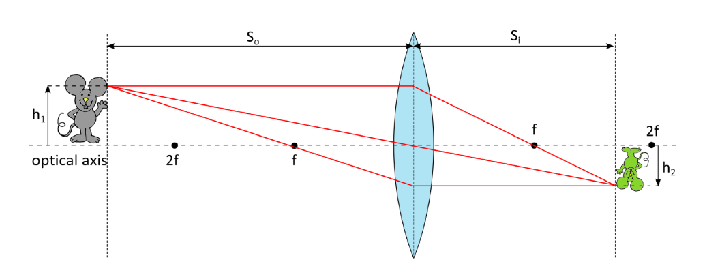
\includegraphics{image_forming_basics.eps}
\caption{Simple image formation using one lens. 
The focal length of the thin lens is $f$, object distance is $s_o$ and image distance is $s_i$. 
The upper ray (parallel to the optical axis on the left) passes through the focal point (denoted as a dot) on the right side of the lens, the middle ray (passing through the centre of the lens) is unrefracted, and the lower ray passes through the focal point on the left side of the lens, and comes out parallel to the optical axis on the other side. 
}
\label{fig:imageforming}
\end{figure}

As the distance between the object and lens ($s_o$) is varied, the distance between the lens and image ($s_i$) also changes. This relationship is determined by the lens focal length ($f$) using the thin lens equation.

\begin{equation}
\frac{1}{s_o} + \frac{1}{s_i} = \frac{1}{f}
\label{eq:thinlens}
\end{equation}

The following conventions are used: $f>0$ for convex lenses, $f<0$ for concave lenses, $s_o$ is always $>0$, $s_i>0$ for real images, and $s_i<0$ for virtual images.
Transverse distances above the optical axis are $>0$. Distance below are negative. 

\vspace{2em}
First of all, you should practice drawing ray diagrams by hand. 
You will need to do this later to explain what you observe on the bench.
Make your diagram big, use all of an A4 sheet of paper. 
By convention, the object is is an upright arrow rather than a grey mouse.
Draw the three cardinal rays:
\begin{itemize}
\item The ray parallel to the optical axis goes through $f$ on the image side.
\item The ray that passes through the centre of the lens travels undeflected.
\item Finally, the ray that goes through $f$ on the object side leaves the lens parallel to the optical axis on the image side. 
\end{itemize}




\clearpage




\subsubsection{1. Determine the focal length of a convex lens }
For the next few exercises you will use an LED as both a light source and an object to image.
You will form various images of the LED emitter. 
Your first task is to set up the LED on the optical rail:

\begin{itemize}
\item Attach a post holder to a rail carriage (Fig.~\ref{fig:post}) and place this on the rail. 
\item Place the LED in the SM1 holder and attach this to a cage plate (CP02) and mount this on a 50~mm post. 
\item Mount the post to your post-holder and place the LED at one end of the rail.
\item Power the LED (remembering to use the current-limiting resistor). 
\end{itemize}


\begin{figure}[h]
\center
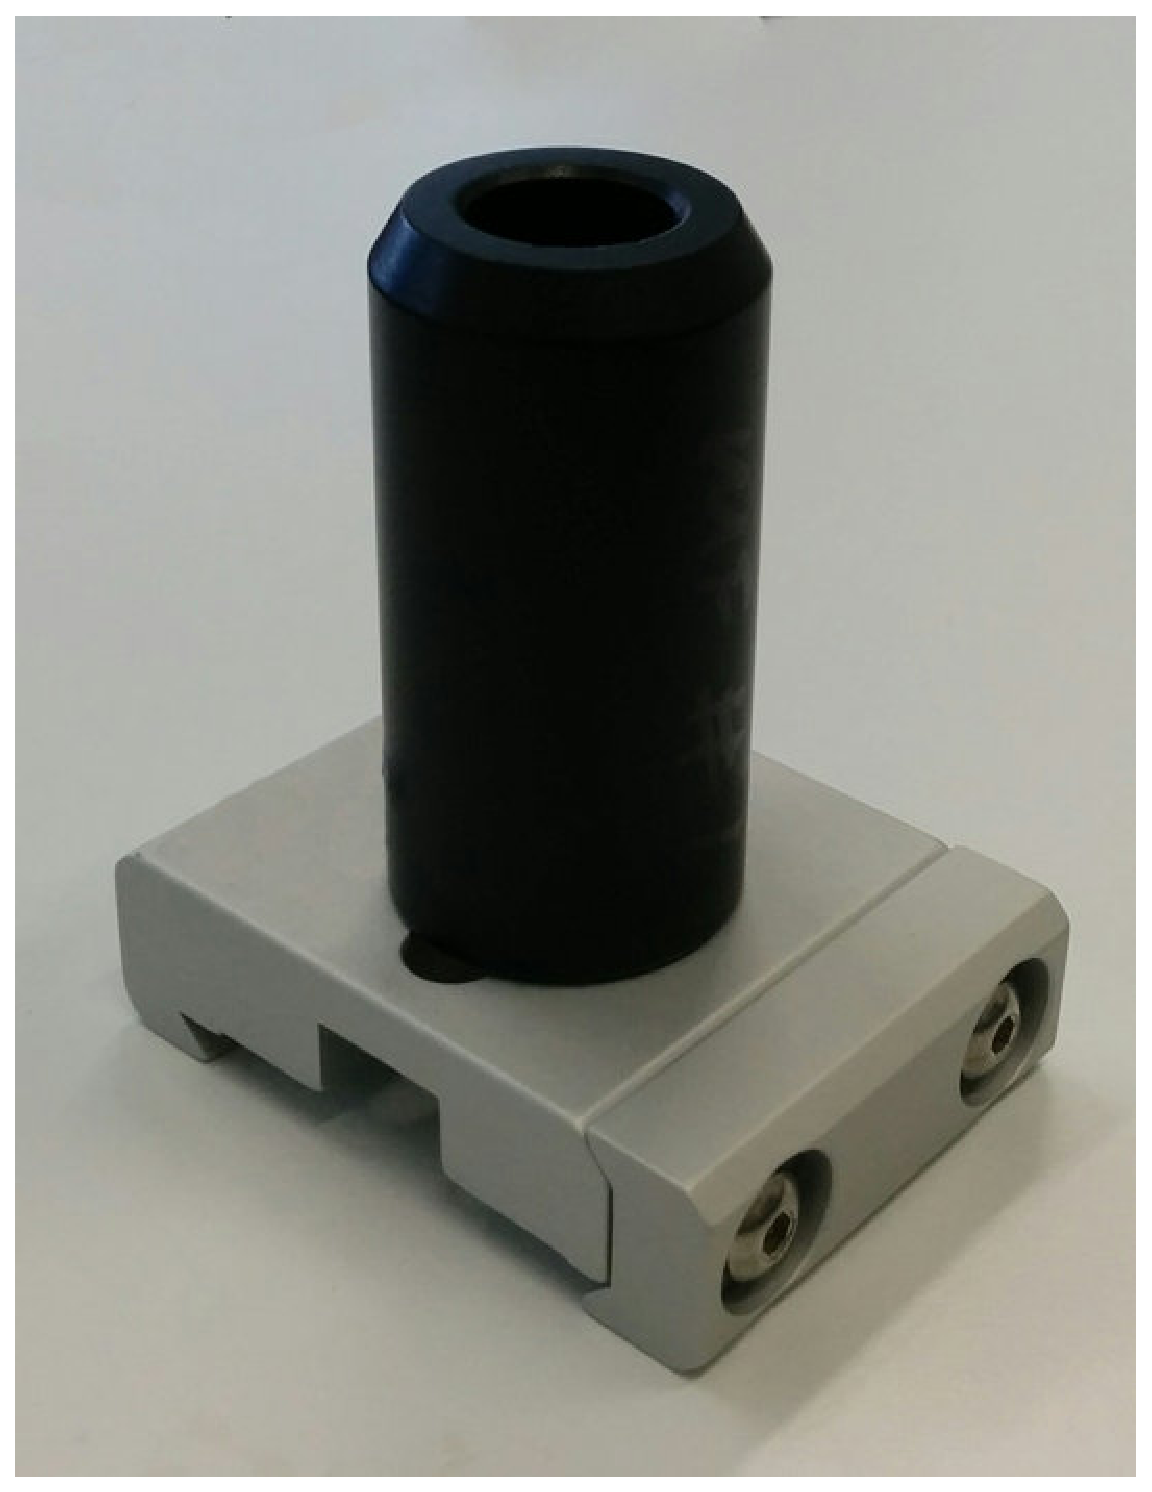
\includegraphics[width=1in]{post_mounted.eps}
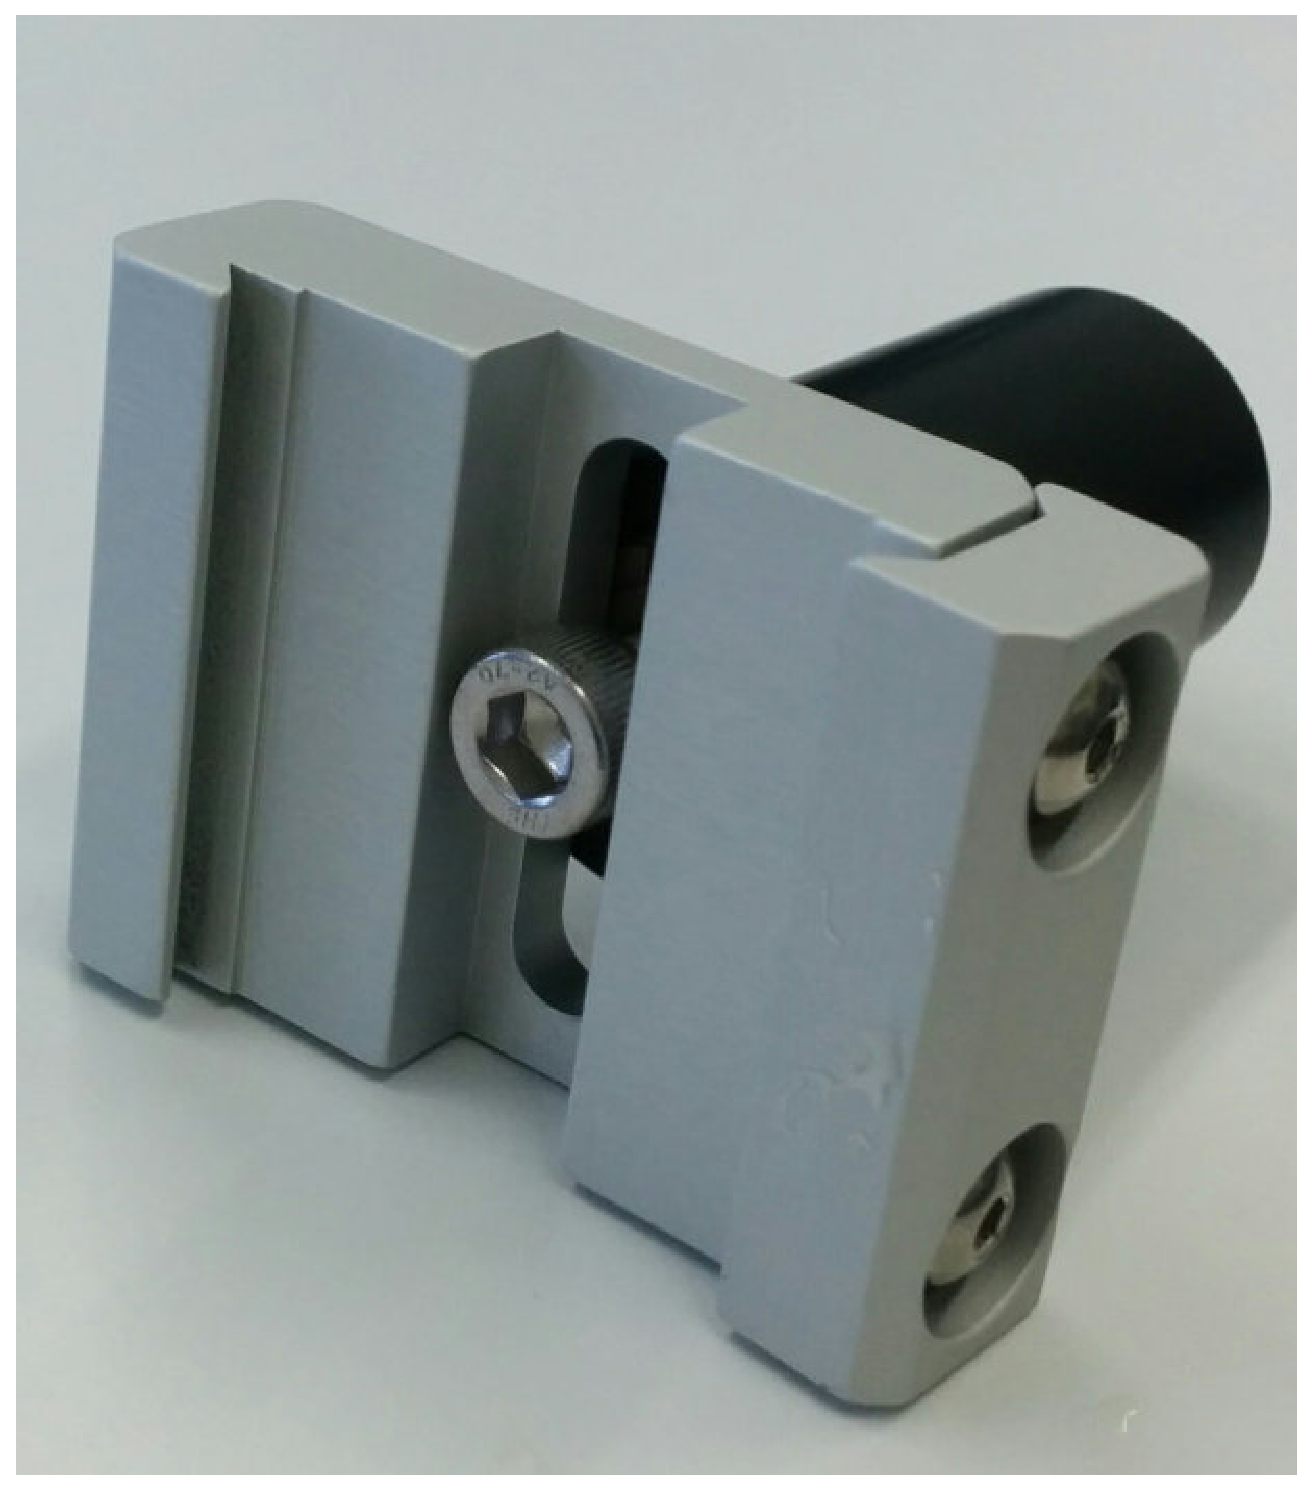
\includegraphics[width=1in]{post_mounted_underside.eps}
\caption{A post holder bolted to a rail carriage.}
\label{fig:post}
\end{figure}

Now choose a lens with a focal length of about $f=100~mm$ and attach the lens to a lens holder using the lens wrench and a retaining ring (this should already be in the lens holder).
Mount the lens on another carriage and attach to the rail next to the LED, allowing the light to go through the lens. 
Try to get the LED aligned with the middle of the lens (precise alignment isn't important). 

You will use this lens to form an image of the LED.
This is called \textbf{finite conjugate} imaging because the image is paired (i.e. conjugated) with an object at a finite distance from it.
The image and sample planes are said to be \textbf{conjugate planes}.
You will be able to form an image on a piece of card or paper if the distance between the lens and LED ($s_o$) is $>1f$.
The image will be of the LED emitter and usually looks like a small bright square, often with fine lines going across it. 
If all you see is a blur, you have not formed an image.

\begin{itemize}
\item Place the lens $<1f$ from the LED and use a piece of card on the other side of the lens to verify that no image is formed at any distance from the lens.
\item Why is no image formed? 
Hint: draw a diagram with two rays: the undeflected ray and the ray coming out parallel with the optical axis and then going through $1f$ on the image side. 
How do the rays behave after they have passed through the lens?
\item Verify that an image is formed when the lens is $>1f$ from the LED: place a card very far from the LED (e.g. at $20f$) and slowly move the lens away from the LED. 
What is the distance between the LED and the lens at which you see an image? 
It should be just over $1f$.
\item Measure $s_i$ for three values of $s_o$ and fill in the table below. 
Using equation~\ref{eq:thinlens}, calculate $f$ for each value of $s_o$.
\item What is the value of $s_i$ when $s_o=2$?
\end{itemize}

\vspace{2em}
\begin{tabular}{| p{1cm} | p{1cm} | p{1cm} |}
\hline
 $s_o$  &  $s_i$  &  $f$  \\
\hline
\hline
 & & \\ \hline
 & & \\ \hline
 & & \\ \hline
\end{tabular}


\subsubsection{2. Magnifying the image}
As you probably noticed, the size of the image of the LED emitter varied with $s_o$.
A lens produces images of different magnifications depending on $s_o$; an image can always be formed when $s_o>f$. 
The magnification of a lens is calculated as follows:

\begin{equation}
M = \frac{h_i}{h_o} = -\frac{s_i}{s_o} = \frac{f}{f-s_o}
\label{eq:mag}
\end{equation}

A value of $M=1$ would mean unitary magnification (the image is the same size as the object). 
Negative numbers indicate an inverted image.

To begin thinking about magnification, hand-draw the ray diagram (as in Fig.~\ref{fig:imageforming}) for the smallest and largest values of $s_o$ that you used above. 
Make sure to give yourself plenty of room. 
Hint: You will run out of paper if you use values too close $1f$.
If you're stuck, choose $1.5f$ and $4f$.
Note the changing angles of the rays and how they lead to different image sizes as $s_o$ changes. 
We will now demonstrate magnification in a slightly different way:

\begin{itemize}
\item Mount a lens of about $f=60~mm$ in a holder and attach a post to it. 
Go over to the window and form an image of the outside world on a piece of paper. 
The image is formed at $1f$, as you already know. 
\item Repeat with a lens of about $f=100~mm$ lens. 
What two things do you notice about the image? 
\item Fig.~\ref{fig:outside} models the situation you saw. Satisfy yourself that this provides a reasonable explanation. 
If you wish, you can use the Chrome Ray Optics Simulator to make your own ray diagram of this imaging condition. 
\item Go back to the lens and LED.
Calculate the values of $s_o$ and $s_i$ which produce $M=-4$ (remember, negative just means inverted) for a $f=100~mm$ lens. 
Measure the size of the LED image and so calculate the size of the LED emitter. 
Hint: you don't need to set up the lens to yield exactly $M=-4$, just get it approximately there and measure $s_i$ and $s_o$.
\item Remember the value of $s_i$ when $s_o=2f$? Therefore what is $M$ when $s_o=2f$?
\end{itemize}


\begin{figure}[h]
\center
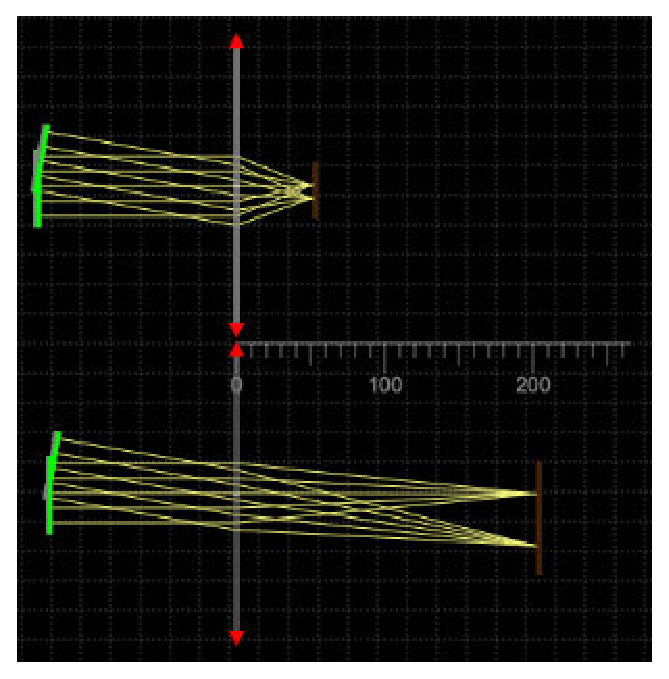
\includegraphics[width=2.5in]{image_forming_outside.eps}
\caption{Images formed at $1f$ from light originating at infinity. 
The top is a $f=50~mm$ lens and the bottom a $f=200~mm$ lens.
Light from different regions of the object arrive in parallel rays that come in at different angles. 
Each set of parallel rays come into focus at a point, satisfying the image-forming condition. 
In the longer focal length lens, these points are further apart than in the shorter focal length lens. 
Thus, the longer focal length lens magnifies the image to a greater degree. 
 }
\label{fig:outside}
\end{figure}


What you have covered above demonstrates an important property of lenses: that they work the same both forwards and backwards.
Recall the definition of an image-forming condition: \textbf{light rays leaving one point (or region) of the object arrive at some other defined point (or region)}.
This is why no image was formed when the LED was at $s_o=f$, since rays leaving the lens are parallel and do not converge on the other side. 
However, you \textit{were} able to form an image at $s_i=f$ when the object was very far away. 
The ray diagrams of these two conditions are \textit{identical}--the only difference is that the object is at $1f$ in the first case and at infinity in the second case.

\subsubsection{3. Virtual images}
At distances $s_o<f$, you were unable to form an image of the sample on the card because the rays emerging from the other side \textit{diverged}.
\begin{itemize}
\item Place the LED at $0.5f$ from a lens of your choice. 
\item See how the light diverges coming out of the lens. 
\item Draw the ray diagram for this scenario: Place an object at about $0.5f$.
Draw the ray that leaves the tip of the object and continues undeflected through the middle of the lens. 
Draw the ray that travels parallel to the optical axis and goes through $1f$ on the other side.
See how these rays diverge. 
\end{itemize}

It would seem that no image is formed yet, surprisingly, a \textit{virtual image} is formed on the same side of the lens as the object. 
This may sound like a peculiar concept, but you are already familiar with virtual images as this is how you see images in flat mirrors (Fig.~\ref{fig:mirror}). 
The extended rays in the case of the mirror can be created from the \textit{diverging} rays from the object. 
In the case of the the lens at $s_o<f$ we also have diverging rays and so can also draw extended rays as we did for the mirror. 
Add the extended rays to your ray diagram by continuing the rays on the object side of the lens until they converge. 
Where do they converge? 
What does this tell you about the magnification of the virtual image?
You have made a magnifying glass!
Verify this by using your lens to magnify your notebook (lenses of about $f=100~mm$ to $f=50~mm$ work best).
\begin{figure}[h]
\center
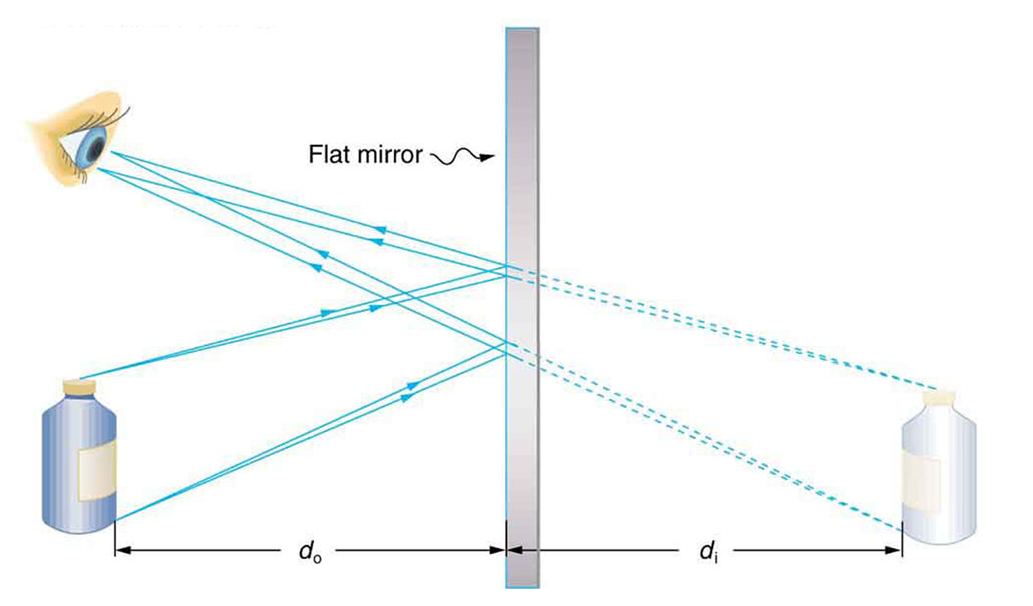
\includegraphics[width=4in]{virtual_image_mirr.eps}
\caption{A virtual image of the bottle is created on the far side of the mirror. 
This is described by the dotted lines which are `extended rays' that are used to form the virtual image. }
\label{fig:mirror}
\end{figure}

A virtual image is also formed by a negative (concanve) lens, as shown in Fig.~\ref{fig:neglens}). 
Examine the ray diagram of the negative lens. 
What do you predict you will see if you look through a negative lens?
Verify this (the negative lens in your kit has a negative focal length number written on the box). 
\begin{figure}[h]
\center
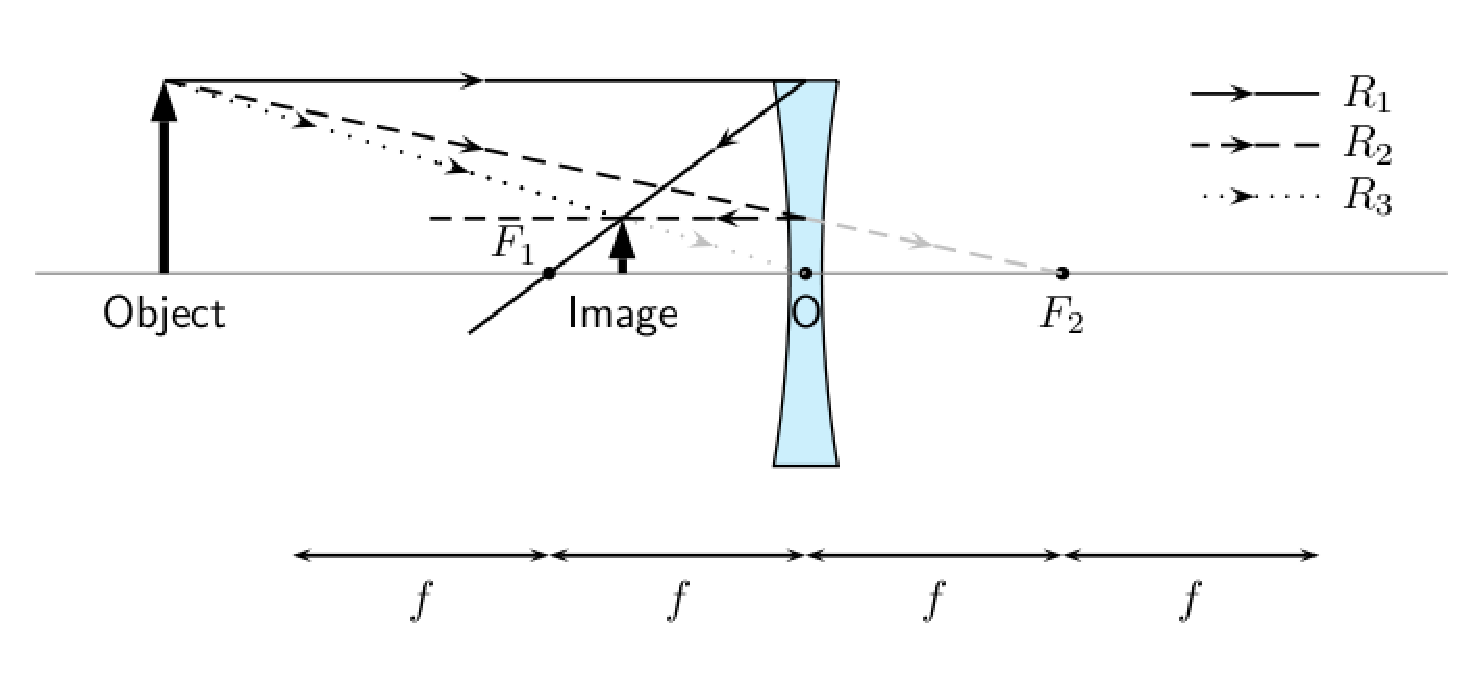
\includegraphics[width=3in]{negative_lens.eps}
\caption{Ray diagram of a negative lens.}
\label{fig:neglens}
\end{figure}

In summary, a \textbf{real image} is formed on the opposite side of the lens to the sample. 
This allows the detector to be physically separated from the sample, which is rather useful.
A \textbf{virtual image} is formed on the \textit{same} side of the lens as the object. 

\clearpage

\subsection{Infinite Conjugate}
The \textbf{infinite conjugate} refers to the situation where the object is located at a distance of $1f$ from a lens (Fig.~\ref{infiniteConjugate}). 
In this scenario the rays leaving the lens are parallel and do not converge, so this is not an image forming condition. 
Instead, the image can be considered to be infinitely far away (hence the name). 
If a second lens is added, then an image can be formed. 
The magnification of the image is defined as Eq.~\ref{eq:magIC}. 
This arrangement is useful because the image is always formed at $1f$ from the second lens irrespective of the distance between the lenses.
Most microscope objectives are designed to work in this configuration since it allows filters to be added into the infinite space without altering the location of the image plane. 
Such objectives are known as `infinity corrected`, since they are designed to produce their best images with the sample at $1f$.

\begin{equation}
M=-\frac{f_2}{f_1}
\label{eq:magIC}
\end{equation}

\begin{figure}[h]
\center
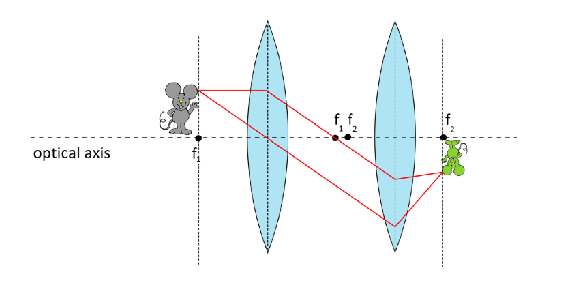
\includegraphics[width=4in]{infiniteConjugate.eps}
\caption{The infinite conjugate.}
\label{infiniteConjugate}
\end{figure}

\begin{itemize}
\item Set up two lenses with different focal lengths on the rail to build the infinite conjugate. 
Place the LED at the $f$ of the first lens before placing the second lens. 
\item Place a screen at the $f$ of the second and hold it in place with the post-mounted clip.
\item Verify the consequences of the infinite space by moving the second lens and maintaining the screen at $f$ of the second lens. 
What happens to the image size?
\item Swap the first lens with one of a different focal length. 
Verify that the image size changes in the manner in which you expect.
Hint: the easiest way of doing this to place the screen at the far end of the rail, the second lens $1f$ from the screen, then swap the first lens and move it back and forth to focus. 
\end{itemize}

\clearpage
\subsection{Beam expanders}
Lenses can be used to expand the diameter of a light beam, such a laser.
Expanders can be built using either two convex lenses (Fig.~\ref{beamExpander1}) or a convex and concave lens (Fig.~\ref{beamExpander2}). 
In both cases the lenses are set up such that their focal points coincide (i.e. they are separated by the sum of their focal lengths). 
The degree to which a beam is expanded can be calculated as:
\begin{equation}
\frac{d_2}{d_1}=\frac{f_2}{f_1}
\label{eq:beamExp}
\end{equation}

\begin{figure}[h]
\center
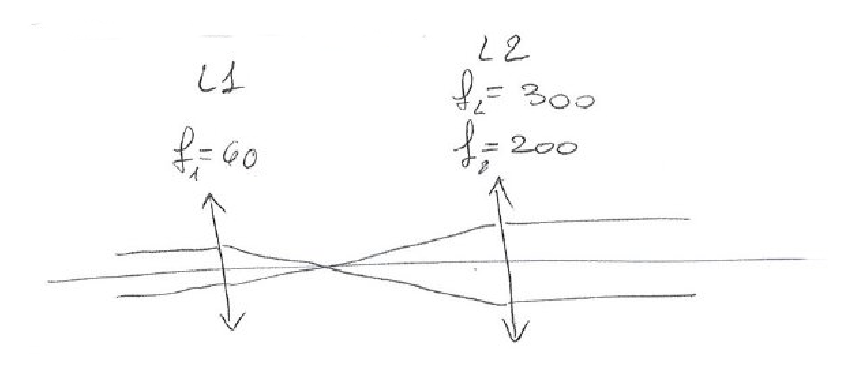
\includegraphics[width=4.5in]{beamExpander1.eps}
\caption{Beam expander with two convex lenses.}
\label{beamExpander1}
\end{figure}

\begin{figure}[h]
\center
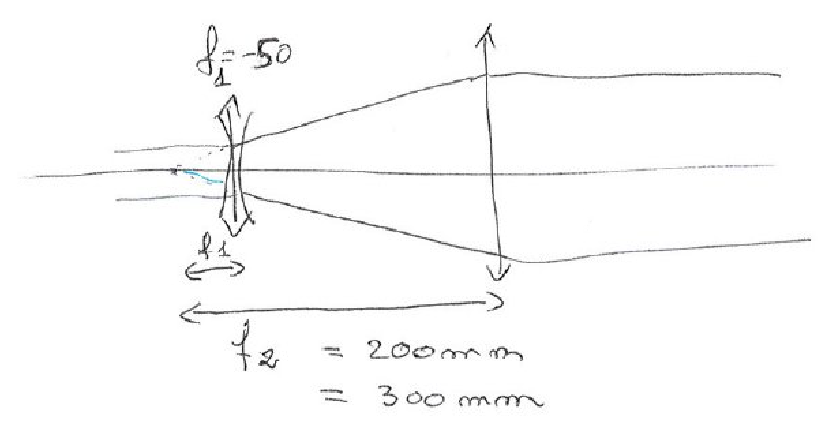
\includegraphics[width=4.5in]{beamExpander2.eps}
\caption{Beam expander with one convex and one concave lens.}
\label{beamExpander2}
\end{figure}

To explore beam expanders you will you will use a laser as a light source instead of an LED. 
This is because we want collimated light (parallel rays) entering the system. 
You will first need to clamp your laser pointer and align it to the rail:

\begin{itemize}
\item Clamp your laser pointer to the top of a post using the RA90 post clamp. 
\item Place the pointer at one end of the rail and align it such that it points straight down the rail to the other end. 
\item Attach an iris to a post that is of suitable length to place the iris at the same height as the laser pointer. 
\item Place the iris next to the laser pointer, close it and adjust the height of the laser pointer so the beam goes through the hole. 
\item Move the iris to the other end of the rail. 
\item Rotate the post the laser pointer sits on and change the clamping force until the beam goes through the iris. 
Do not translate the laser pointer up and down.
\item The beam should now be traveling more or less parallel with the rail. 
\end{itemize}

Now you're ready to build some expanders:

\begin{itemize}
\item Construct a beam expander using a $f=300~mm$ lens and an $f=100~mm$ lens.
Make sure that the two focal points coincide by checking that the exit beam remains collimated (does not diverge or converge)
at all distances from the second lens. 
\item Measure the size of the expanded beam and so calculate size of the unexpanded beam.
\item Swap out the $f=100~mm$ lens with the $f=-50~mm$ convex lens. Verify that the expanded beam diameter doubles. 
What advantages does the negative lens add?
\item Build a beam expander to yield the maximum magnification your optics kit allows (e.g. $f=300~mm$ and $f=30~mm$ to yield 10x). 
The beam expander you have built also goes by another common name.  What is it? 
Hint: think about what happens to beams that do not travel on-axis (Fig.~\ref{fig:telescope}).
Once you've figured it out, remove the laser pointer and use your device. 
\end{itemize}


\begin{figure}[h]
\center
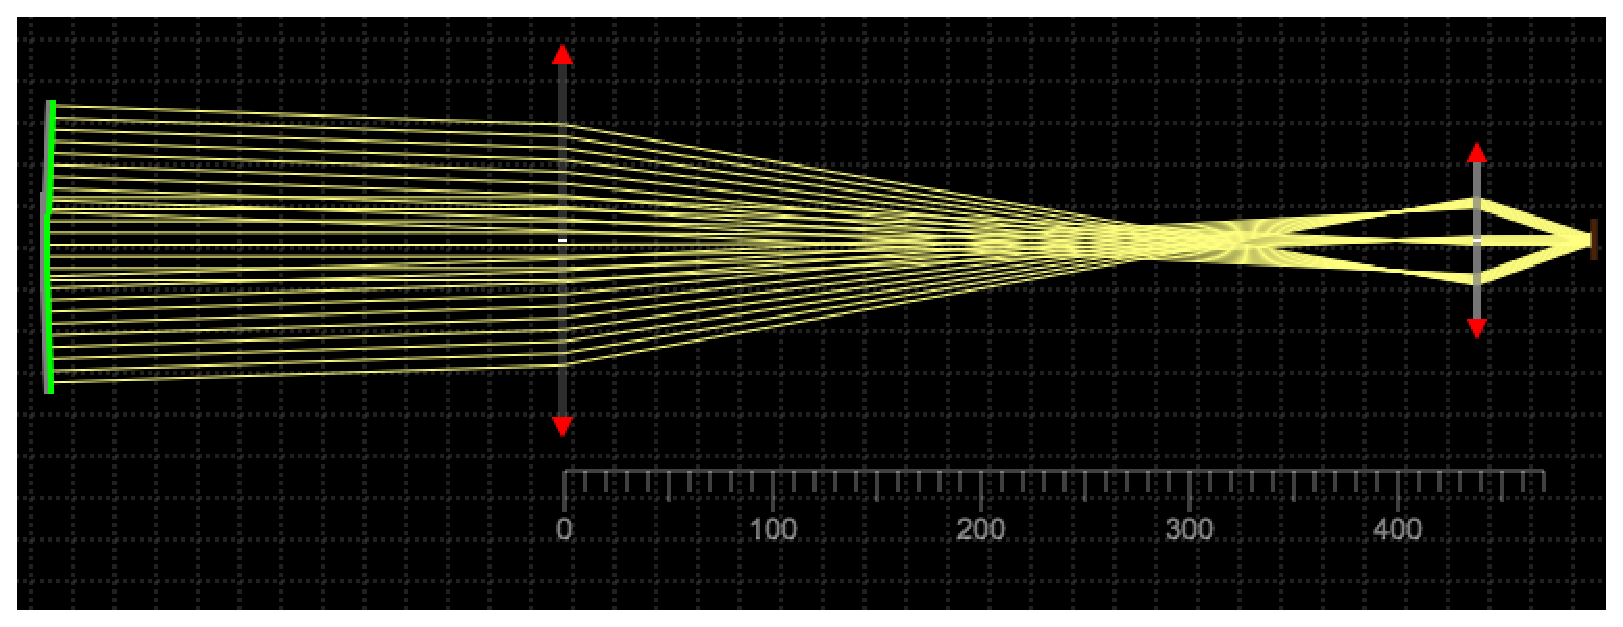
\includegraphics[width=4.5in]{telescope_ray_diag.eps}
\caption{A beam expander composed of an $f=400~mm$ lens and an $f=40~mm$ lens. 
In addition to the collimated beam arriving on-axis, two off-axis beams are shown.}
\label{fig:telescope}
\end{figure}

\clearpage



\subsection{Composite optical elements}
As you will have noticed above, image quality tends to be best in the centre of the field of view and decreases towards the edges. 
A variety of aberrations (Fig.~\ref{fig:aberrations}) are at play and these tend to become progressively worse for light coming in at steeper angles to the optical axis.

\begin{figure}[h]
\center
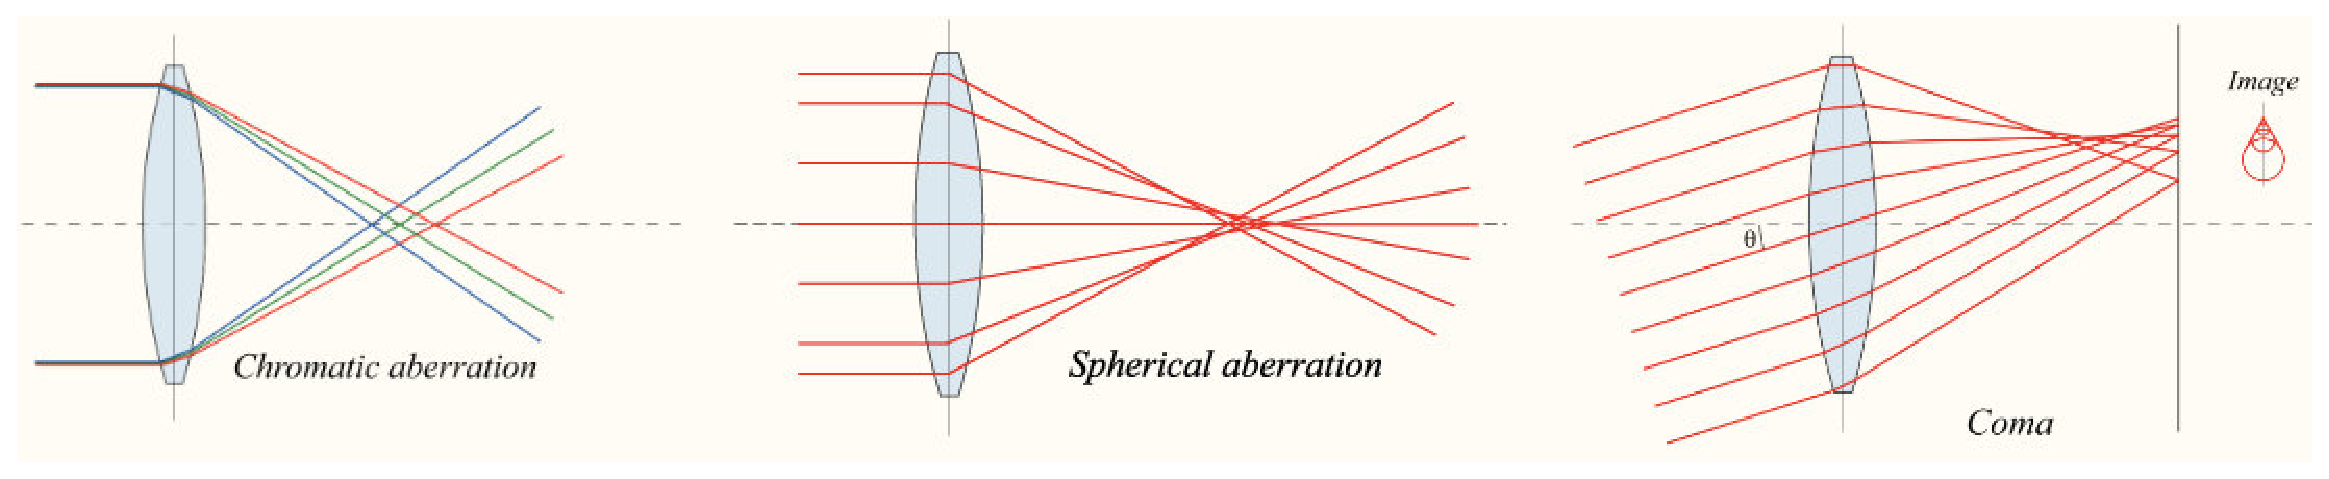
\includegraphics[width=6in]{aberrations.eps}
\caption{The three most common optical aberrations. 
Chromatic aberration sees light of different wavelengths coming into focus at different distances from the lens.
Spherical aberration sees on-axis light coming into focus at different distances from the lens. 
Coma is the situation where off-axis light does not come into focus in the same spot. }
\label{fig:aberrations}
\end{figure}

To correct for this, objectives and eyepieces (Fig.~\ref{fig:composite}) are built by combining multiple lenses in close proximity. 
The purpose of these extra elements is to correct for aberrations given certain constraints. 
For example, most microscope objectives assume the sample is at $1f$; further, they assume a particular immersion medium, presence of a coverslip, etc.
Note that in objectives and eyepieces the light doesn't pass through a focal point within the device and so they can be considered to be a single complex lens.

\begin{figure}[h]
\center
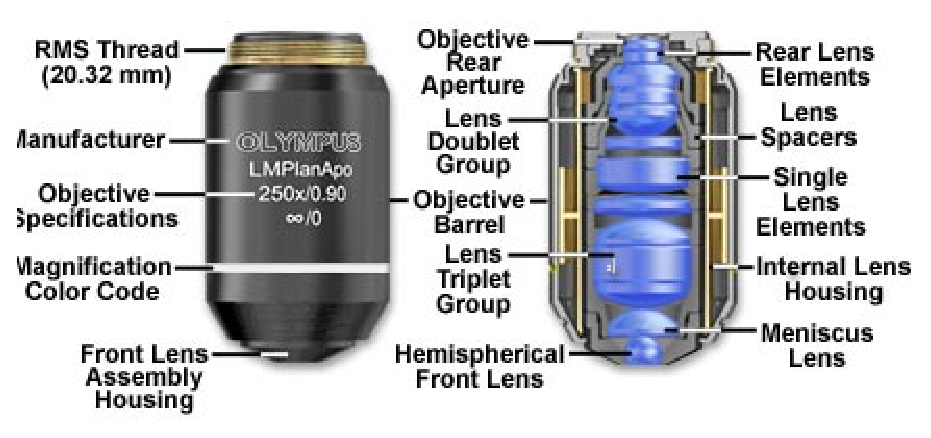
\includegraphics[width=2.8in]{objectivesfigure1.eps}
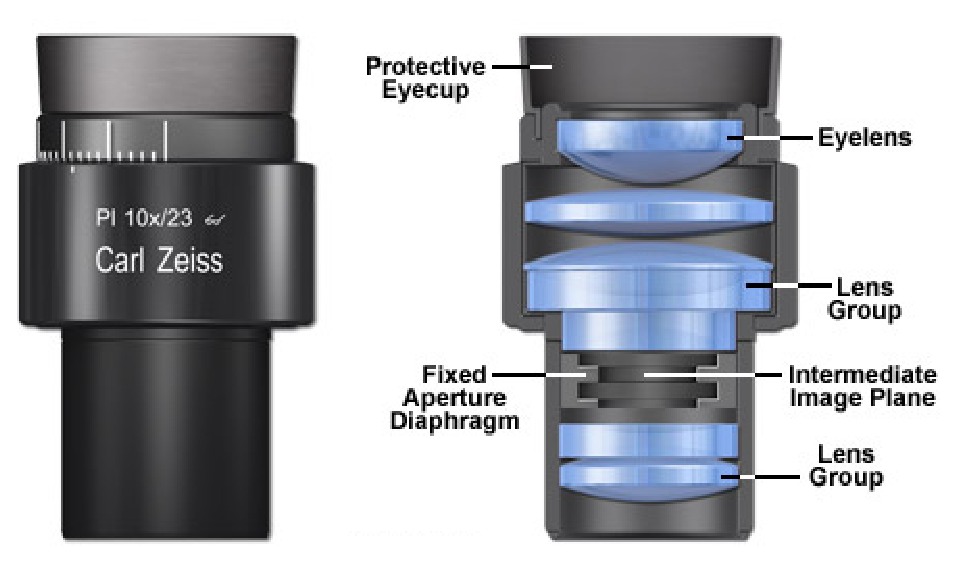
\includegraphics[width=2.2in]{eyepieces5.eps}
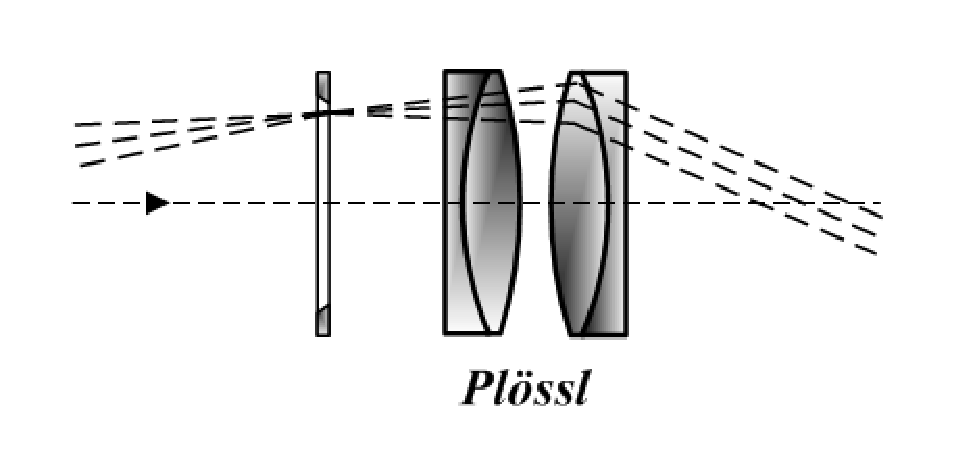
\includegraphics[width=2.2in]{Plossl.eps}
\caption{The composite lens arrangements found in microscope
  objectives (left) and eyepieces (middle).
  The Pl\"{o}ssl eyepiece is composed of two sets of achromatic doublet lenses (bottom).}
\label{fig:composite}
\end{figure}


Here we will experiment with a simple composite optical arrangement: the Pl\"{o}ssl eyepiece (Fig.~\ref{fig:composite}). 
Pl\"{o}ssls are commonly used in amateur astronomy because they are not expensive and provide a relatively wide (50 degree) field of view that is of good 
quality if the eyepiece is well made. 
Pl\"{o}ssls also make suitable scan lenses for two photon microscopy\footnote{Negrean \& Mansvelder, 2014, PMID: 24877017}.
You will now construct a Pl\"{o}ssl using two $f=60~mm$ singlet lenses.


\begin{itemize}
\item First construct a beam expander ($f_1$=30~mm lens and a $f_2$=300~mm). 
The expanded beam will be directed into your eyepiece, which will make it easier to measure its focal length.
\item Build the Pl\"ossl by placing the two $f=60~mm$ lenses as close as possible with their flat sides facing outwards. 
You might need to move the post holders on the rail carriages to allow the lenses to meet.
Since collimated light leaves your beam expander, you can place the Pl\"ossl at any distance from the $f=30~mm$ lens. 
\item Verify that your Pl\"{o}ssl behaves more or less as expected: 
Eq.~\ref{eq:compoundLensF} gives the distance between the middle of the compound lens and the focal point. 
\item Separate your lens elements by about 15~mm and measure and measure the change in focal length.
\end{itemize}

The effective focal length of two thin lenses are separated in air by some distance $d$ is given by
\begin{equation}
\frac{1}{f} = \frac{1}{f_1} + \frac{1}{f_2} - \frac{d}{f_1f_2}
\label{eq:compoundLensF}
\end{equation}

A telescope built from two positive lenses is known Keplerian telescope. 
A Galilean telescope uses a negative lens as the eyepiece and forms a non-inverted image.
Build a Keplerian telescope using $f=300~mm$ singlet lens for the objective and a $30~mm$ lens for the eyepiece. 
Look through it familiarise yourself with what the image looks like then replace the eyepiece with your Pl\"{o}ssl. 
The magnification will similar, but the image quality should be better. 
The apparent field of view should be wider and there will be substantially less pincushion distortion. 
You will still see chromatic aberration. 
If you have an achromatic $f=300~mm$ doublet, then you can swap this in and see the reduction in chromatic aberration and a sharper image. 
Your telescope is just powerful enough to see the moons of Jupiter. 


\subsection{Optics Challenge}
Arrange 4 lenses so as to form a de-magnified, real, upright
image. Hints: 
\begin{itemize}
\item Use one negative lens.
\item Space will be a problem: the lenses will take up the whole rail
  and so you will need to place the target and screen outside of the
  rail. 
\item Use the light-guide to illuminate your target to avoid it
  becoming too dim. 
\item There are multiple solutions to this problem.
\end{itemize}


\clearpage
\section{Illuminating the sample}
Different samples are best illuminated in different ways.
In transmission microscopy the sample is illuminated from the opposite side to which it is imaged. 
In fluorescence microscopy the sample is illuminated from the same side, with the objective also serving as the condenser. 
It is not efficient to illuminate the sample directly (with no intervening lenses) because light is emitted in all directions from the source but only a narrow range of ray angles reach the specimen. 
In the following two exercises you will build two different illumination systems: critical and K\"{o}hler. 
The exercises may work better if you use a laser to align the lenses before switching to the LED for imaging the sample. 


\subsubsection{B. Building a telescope}
\begin{itemize}
\item Draw an arrow on a coverslip to use as an target to image. 
\item Use a light-guide as a light source with which to illuminate the arrow from behind. 
Use two convex lenses (60~mm and 100~mm, it's up to you which you place nearer the light source and which you place further away). 
\item Put the coverslip at a distance of 150~mm from the first lens, between the lens and the light source. 
Separate the lenses by 250~mm. 
\item Trace the ray diagram. Where will the image be formed? Is the image inverted?  Verify this experimentally. 
\item Move the lenses to alter their relative distance. In which condition is the image virtual? In
which condition real and inverted? In which condition is no image formed?
\end{itemize}


\subsection{Critical illumination of a sample}
TODO: one lens, then two
In critical illumination the light source is focused onto the specimen (Fig.~\ref{critIlum}).
This may be done with just one lens, although here we will do it with two. 
Use an LED as the light source. 
Build the condenser using two lenses and place the sample at
their focal point. The lens nearer the LED is known as the
\textbf{collector lens} and the lens nearer the sample is known as the
\textbf{condenser lens}. Use the 30 mm for the collector lens and the
60 mm (convex) for the condenser lens. A suitable sample is a
coverslip with thin lines drawn on with a marker. Place the sample at
the focal point of the condenser lens. Use two more lenses to form an
image of the specimen on a piece of card. The \textbf{objective lens}
($f$=100~mm) follows the specimen, and finally the \textbf{tube lens}
($f$=300~mm) is used to form an image. Set up the lenses and image the
image the sample. What problem do you notice?

Critical illumination can be set up using either a finite or an
infinite conjugate image of the light source. A diaphragm (the
`\textbf{aperture diaphragm}') can be placed between the collector and
condenser lens, at the focal point of the second lens (the condenser
lens) to stop down the range of angles reaching the sample. This
allows the NA of the illuminant to be regulated, providing control
over the resolution, contrast, and depth of field. Add the aperture
diaphragm and observe the effect of regulating the aperture on your
sample image. Does the area illuminated alter when the diaphragm is
closed down?

\begin{figure}[h]
\center
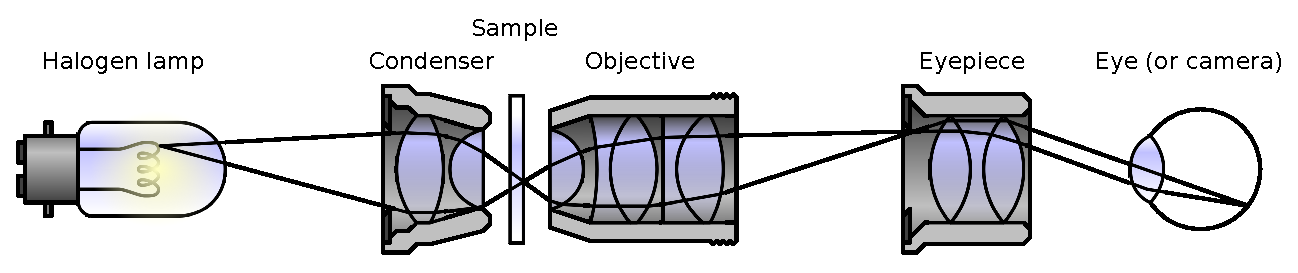
\includegraphics[width=5in]{Critical_Illumination.eps}
\caption{A simple critical illumination set up for visual microscopy.}
\label{critIlum}
\end{figure}


\subsection{K\"{o}hler Illumination}
K\"{o}hler illumination is an important and commonly used technique in
light microscopy, as it provides even illumination of the sample
whilst ensuring the light source (e.g. the bulb filament) is not
visible. This is achieved by adding a third lens (you will use a
$f$=100) so that the image of the filament doesn't appear on the
sample but on the aperture diaphragm (which is the diaphragm located
immediately before the condenser lens). This arrangement not only
permits uniform illumination but also allows a second diaphragm to be
added. This \textbf{field diaphragm} is imaged onto the sample and so
provides a means of regulating the area of illumination. In summary,
whilst an image of the filament is still formed, it occurs at a
different plane to the image formed by the sample. Consequently, when
observing the sample the light source image is out of focus.

You will now convert the critical illumination to K\"{o}hler
illumination.  The components will be arranged in the following order:
\begin{enumerate}
\item Collector lens ($f$=30)
\item Field diaphragm
\item Field lens ($f$=100)
\item Aperture diaphragm
\item Condenser lens ($f$=60)
\item The objective and tube lenses will be as before. 
\end{enumerate}

Again, you will place the LED at one focal length before the collector
lens and the sample at the focal length of the condenser lens. The
arrangement of the components is shown in Fig.~\ref{koehler}. Verify
that you can alter the depth of field by obtaining a second coverslip
and drawing a differet target on it. Stack this alongside the original
sample and vary the sizes of the diaphragms to observe the effects. 


\begin{figure}[h]
\center
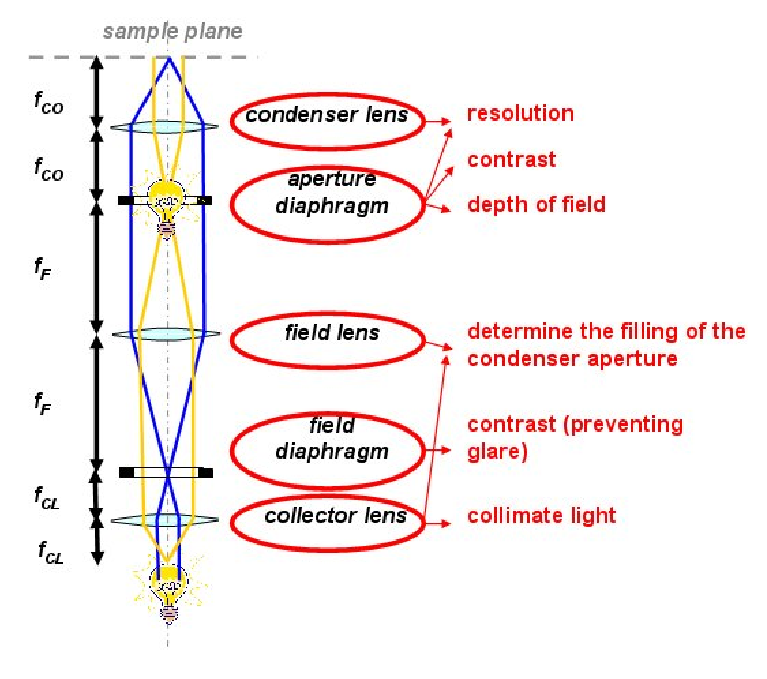
\includegraphics[width=5in]{koehler.eps}
\caption{K\"{o}hler Illumination}
\label{koehler}
\end{figure}




\end{document}
